\documentclass[12pt,a4paper]{article}
\usepackage{cmap} % Makes the PDF copiable. See http://tex.stackexchange.com/a/64198/25761
\usepackage[T1]{fontenc}
\usepackage[brazil]{babel}
\usepackage[utf8]{inputenc}
\usepackage{amsmath}
\usepackage{amsfonts}
\usepackage{amssymb}
\usepackage{amsthm}
\usepackage{textcomp} % \degree
\usepackage{gensymb} % \degree
\usepackage[usenames,svgnames,dvipsnames]{xcolor}
\usepackage{hyperref}
\usepackage{multicol}
\usepackage{graphicx}
\usepackage[margin=2cm]{geometry}

\hypersetup{
    colorlinks = true,
    allcolors = {blue}
}
\usepackage{cancel}

% TODO: Consider using exsheets
% http://linorg.usp.br/CTAN/macros/latex/contrib/exsheets/exsheets_en.pdf
%
% http://ctan.org/tex-archive/macros/latex/contrib/exercise/
% Options: answerdelayed,lastexercise,noanswer
\usepackage[answerdelayed,lastexercise]{exercise}

\addto\captionsbrazil{%
\def\listexercisename{Lista de exerc\'icios}%
\def\ExerciseName{Exerc\'icio}%
\def\AnswerName{Solu\c{c}\~ao do exerc\'icio}%
\def\ExerciseListName{Ex.}%
\def\AnswerListName{Solu\c{c}\~ao}%
\def\ExePartName{Parte}%
\def\ArticleOf{de\ }%
}

\renewcommand{\ExerciseHeaderTitle}{(\ExerciseTitle)\ }
\renewcommand{\ExerciseListHeader}{%\ExerciseHeaderDifficulty%
\textbf{%\ExerciseListName\
\ExerciseHeaderNB.\ %
%\ --- \
\ExerciseHeaderTitle}%
%\ExerciseHeaderOrigin
\ignorespaces}
\renewcommand{\AnswerListHeader}{\textbf{\ExerciseHeaderNB.\ (\AnswerListName)\ }}

\newcommand*\sen{\operatorname{sen}}
\newcommand*\dom[1]{\operatorname{Dom}\left(#1\right)}

\renewcommand{\theenumi}{\alph{enumi}}
\renewcommand\labelenumi{(\theenumi) }

\newcommand*\tipo{Prova III}
\newcommand*\turma{TADS121-01U}
\newcommand*\disciplina{CDI0001}
\newcommand*\eu{Helder G. G. de Lima}
\newcommand*\data{09/06/2018}

\author{\eu}
\title{\tipo - \disciplina}
\date{\data}

\begin{document}
\thispagestyle{empty}
\newgeometry{margin=2cm,bottom=0.5cm}
\begin{center}

\includegraphics[width=9.0cm]{marca} \\
\textbf{\tipo\ (\disciplina / \turma)} \\
Prof. \eu\footnote{
Este é um material de acesso livre distribuído sob os termos da licença \href{https://creativecommons.org/licenses/by-sa/4.0/deed.pt_BR}{Creative Commons BY-SA 4.0}}
\end{center}

\noindent Nome do(a) aluno(a): \underline{\hspace{9,7cm}} Data: \underline{\data}

\begin{center}\fbox{
\begin{minipage}{14cm}

{\footnotesize
\begin{itemize}
\renewcommand{\theenumi}{\Roman{enumi}}
\item Identifique-se em todas as folhas.
\item Mantenha o celular e os demais equipamentos eletrônicos desligados durante a prova.
\item Justifique cada resposta com cálculos ou argumentos baseados na teoria estudada.
\item Resolva (integralmente) apenas os itens de que precisar para somar 10,0 pontos.
\end{itemize}
}

\end{minipage}
}
\end{center}

\begin{ExerciseList}
\Exercise[title={4,0}]
Calcule os limites a seguir utilizando, se possível, as regras de L'Hôpital:
\begin{multicols}{2}
\begin{enumerate}
\item (2,0) $\displaystyle\lim_{x \to 1} \frac{x^{-1} - x^2 + 3x - 3}{(x - 1)^3}$
\item (2,0) $\displaystyle\lim_{x \to 0^{+}} \frac{1}{x} - \frac{1}{\sen(x)}$
\end{enumerate}
\end{multicols}
\Answer
\begin{enumerate}
\item
\[
\lim_{x \to 1} \frac{ \cancelto{0}{x^{-1} - x^2 + 3x - 3} }{ \cancelto{0}{(x - 1)^3}}
\stackrel{\text{L.H.}}{=}\lim_{x \to 1} \frac{ \cancelto{0}{-x^{-2} - 2x + 3} }{ \cancelto{0}{3(x - 1)^2} }
\stackrel{\text{L.H.}}{=}\lim_{x \to 1} \frac{\cancelto{0}{2x^{-3} - 2} }{ \cancelto{0}{6(x - 1) }}
\stackrel{\text{L.H.}}{=}\lim_{x \to 1} \frac{-6x^{-4}}{6}
=-1
\]
\textbf{Solução alternativa:}
\begin{align*}
\lim_{x \to 1} \frac{x^{-1} - x^2 + 3x - 3}{(x - 1)^3}
& = \lim_{x \to 1} \frac{x^{-1} - x^2 + 3x - 3}{x^3 - 3x^2 + 3x -1}
    \cdot \frac{x}{x}
  = \lim_{x \to 1} \frac{\cancelto{0}{1 - x^3 + 3x^2 - 3x}}{\cancelto{0}{x^4 - 3x^3 + 3x^2 -x}} \\
& \stackrel{\text{L.H.}}{=}
    \lim_{x \to 1} \frac{\cancelto{0}{-3x^2 +6x - 3}}{\cancelto{0}{4x^3 - 9x^2 + 6x - 1}}
  \stackrel{\text{L.H.}}{=}
    \lim_{x \to 1} \frac{\cancelto{0}{-6x +6}}{\cancelto{0}{12x^2 - 18x + 6}} \\
& \stackrel{\text{L.H.}}{=}
    \lim_{x \to 1} \frac{-6}{24x - 18}
 = \frac{-6}{24 - 18} = -1
\end{align*}

\item
\begin{align*}
\lim_{x \to 0^{+}} \cancelto{+\infty}{\frac{1}{x}} - \cancelto{+\infty}{\frac{1}{\sen(x)}}
& = \lim_{x \to 0^{+}} \frac{\cancelto{0}{\sen(x) - x}}{\cancelto{0}{x\sen(x)}}
\stackrel{\text{L.H.}}{=} \lim_{x \to 0^{+}} \frac{\cancelto{0}{\cos(x) - 1}}{\cancelto{0}{\sen(x)+x\cos(x)}} \\
& \stackrel{\text{L.H.}}{=} \lim_{x \to 0^{+}} \frac{-\sen(x)}{\cos(x)+\cos(x)-x\sen(x)}
= \frac{0}{2} = 0
\end{align*}
\end{enumerate}


\Exercise[title={2,0}] Supondo que um retângulo tenha $120cm$ de perímetro, responda:
\begin{enumerate}
\item (1,0) É possível que a área deste retângulo seja \textbf{maior} do que a de qualquer outro retângulo de mesmo perímetro? Em caso afirmativo, qual é a área do retângulo?
\item (1,0) É possível que a área deste retângulo seja \textbf{menor} do que a de qualquer outro retângulo de mesmo perímetro? Em caso afirmativo, qual é a área do retângulo?
\end{enumerate}
\Answer Se um retângulo tem lados que medem $x$ e $y$ então seu perímetro é $P = 2x+2y$ e sua área é $A = x \cdot y$. Assim, no caso de um retângulo com $120cm$ de perímetro, tem-se $2x+2y = 120$ e consequentemente $y=60-x$, o que implica que sua área é uma função de $x$, definida por $A(x) = x \cdot( 60 - x ) = 60x - x^2$.
\begin{enumerate}
\item Para que este retângulo tenha uma área maior do que a de qualquer outro retângulo de mesmo perímetro, sua área deve ser o valor máximo da função $A$. Como $A^\prime(x) = 60-2x$, para todo $x$, o único ponto crítico de $A$ ocorre quando $60-2x = 0$, isto é, para $x = 30$. Como $A^{\prime\prime}(x) = -2 < 0$, o ponto crítico $x = 30$ é um ponto de máximo. Assim, a situação descrita no enunciado é possível, desde que os lados do retângulo meçam $x = 30cm$ e $y = 60 - x = 60 - 30 = 30 cm$. Neste caso, a área será dada por $A(30) = 30 \cdot 30  = 900 cm^2$.
\item Pela discussão do item anterior, a função $A$ não possui ponto de mínimo, ou seja, qualquer que seja a área de um retângulo, sempre existirá outros retângulos com áreas ainda menores, e com o mesmo perímetro. De fato, fazendo $x$ tender a zero, resulta que $\lim_{x \to 0} A(x) = \lim_{x \to 0} 60x-x^2 = 0$.
\end{enumerate}

\Exercise[title={4,0}] Seja $f(x) = 3x - 6\sqrt{x}$. Utilize as ferramentas do cálculo diferencial para obter, quando existirem, ou explicar o motivo de não existirem:
\begin{enumerate}
\item (0,5) As derivadas de primeira e segunda ordem da função $f$.
\item (0,5) $\lim_{x \to +\infty} f(x)$.
\item (1,0) Todos os intervalos $(a,b)$ em que a função:
\begin{enumerate}
\item É \textbf{crescente} e \textbf{decrescente}, respectivamente.
\item Tem \textbf{concavidade para cima} e \textbf{para baixo}, respectivamente.
\end{enumerate}
\item (1,0) Todos os pontos do domínio de $f$ que forem considerados \textbf{críticos}, de \textbf{máximo}, de \textbf{mínimo} (locais e globais) e de \textbf{inflexão}. Argumente baseando-se nas respostas anteriores.
\item (1,0) O \textbf{gráfico} da função, usando (corretamente) os dados que encontrou.
\end{enumerate}
\Answer
\begin{enumerate}
\item Tem-se
$f^\prime(x) = 3-\dfrac{3}{\sqrt{x}} = \dfrac{3\sqrt{x}-3}{\sqrt{x}}$
e
$f^{\prime\prime}(x) = \dfrac{3}{2 \sqrt{x^3}}$.
\item  $\displaystyle
\lim_{x \to +\infty} f(x)
= \lim_{x \to +\infty} 3x - 6\sqrt{x}
= \lim_{x \to +\infty} \cancelto{+\infty}{\sqrt{x}}\cancelto{+\infty}{(3\sqrt{x} - 6)}
= +\infty$

\textbf{Solução alternativa:}
\[
\lim_{x \to +\infty} 3x - 6\sqrt{x}
= \lim_{x \to +\infty} (3x - 6\sqrt{x}) \cdot \frac{3x + 6\sqrt{x}}{3x + 6\sqrt{x}}
= \lim_{x \to +\infty} \frac{\cancelto{+\infty}{9x^2 - 36x}}{ \cancelto{+\infty}{3x + 6\sqrt{x}}}
\stackrel{\text{L.H.}}{=}
  \lim_{x \to +\infty} \frac{\cancelto{+\infty}{18x - 36}}{\cancelto{3}{3 + \frac{3}{\sqrt{x}}}}
= +\infty
\]

\item
\begin{enumerate}
\item Considerando que
\[
f^\prime(x) > 0
\Leftrightarrow
\frac{3\sqrt{x}-3}{\sqrt{x}} > 0
\Leftrightarrow
3\sqrt{x}-3 > 0
\Leftrightarrow
3\sqrt{x} > 3
\Leftrightarrow
\sqrt{x} > 1
\Leftrightarrow
x \in (1, +\infty),
\]
conclui-se que $f$ é crescente em $(1, +\infty)$. Analogamente, $f^\prime(x) < 0 \Leftrightarrow x \in (0,1)$, então $f$ é decrescente em $(0,1)$.
\item Como $f^{\prime\prime}(x) = \frac{3}{2 \sqrt{x^3}} > 0$, para todo $x \in \dom{f} = [0,+\infty)$, a concavidade é sempre para cima.
\end{enumerate}
\item Os únicos pontos críticos de $f$ em $[0,+\infty)$ são o ponto $x = 0$, em que a derivada não está definida, e $x = 1$, em que ela se anula. Como $x=0$ é um dos extremos do intervalo e $f$ decresce em $(0,1)$, há um ponto de máximo local em $x = 0$ (que não é global pois, por exemplo, $f(0) = 0 < 9 = f(9)$). Além disso, como $f^{\prime\prime}(1) >0$, há um ponto de mínimo local em $x=1$, que é o ponto de mínimo global. Não existem pontos de inflexão pois a concavidade não muda no domínio de $f$.
\item \
\begin{center}
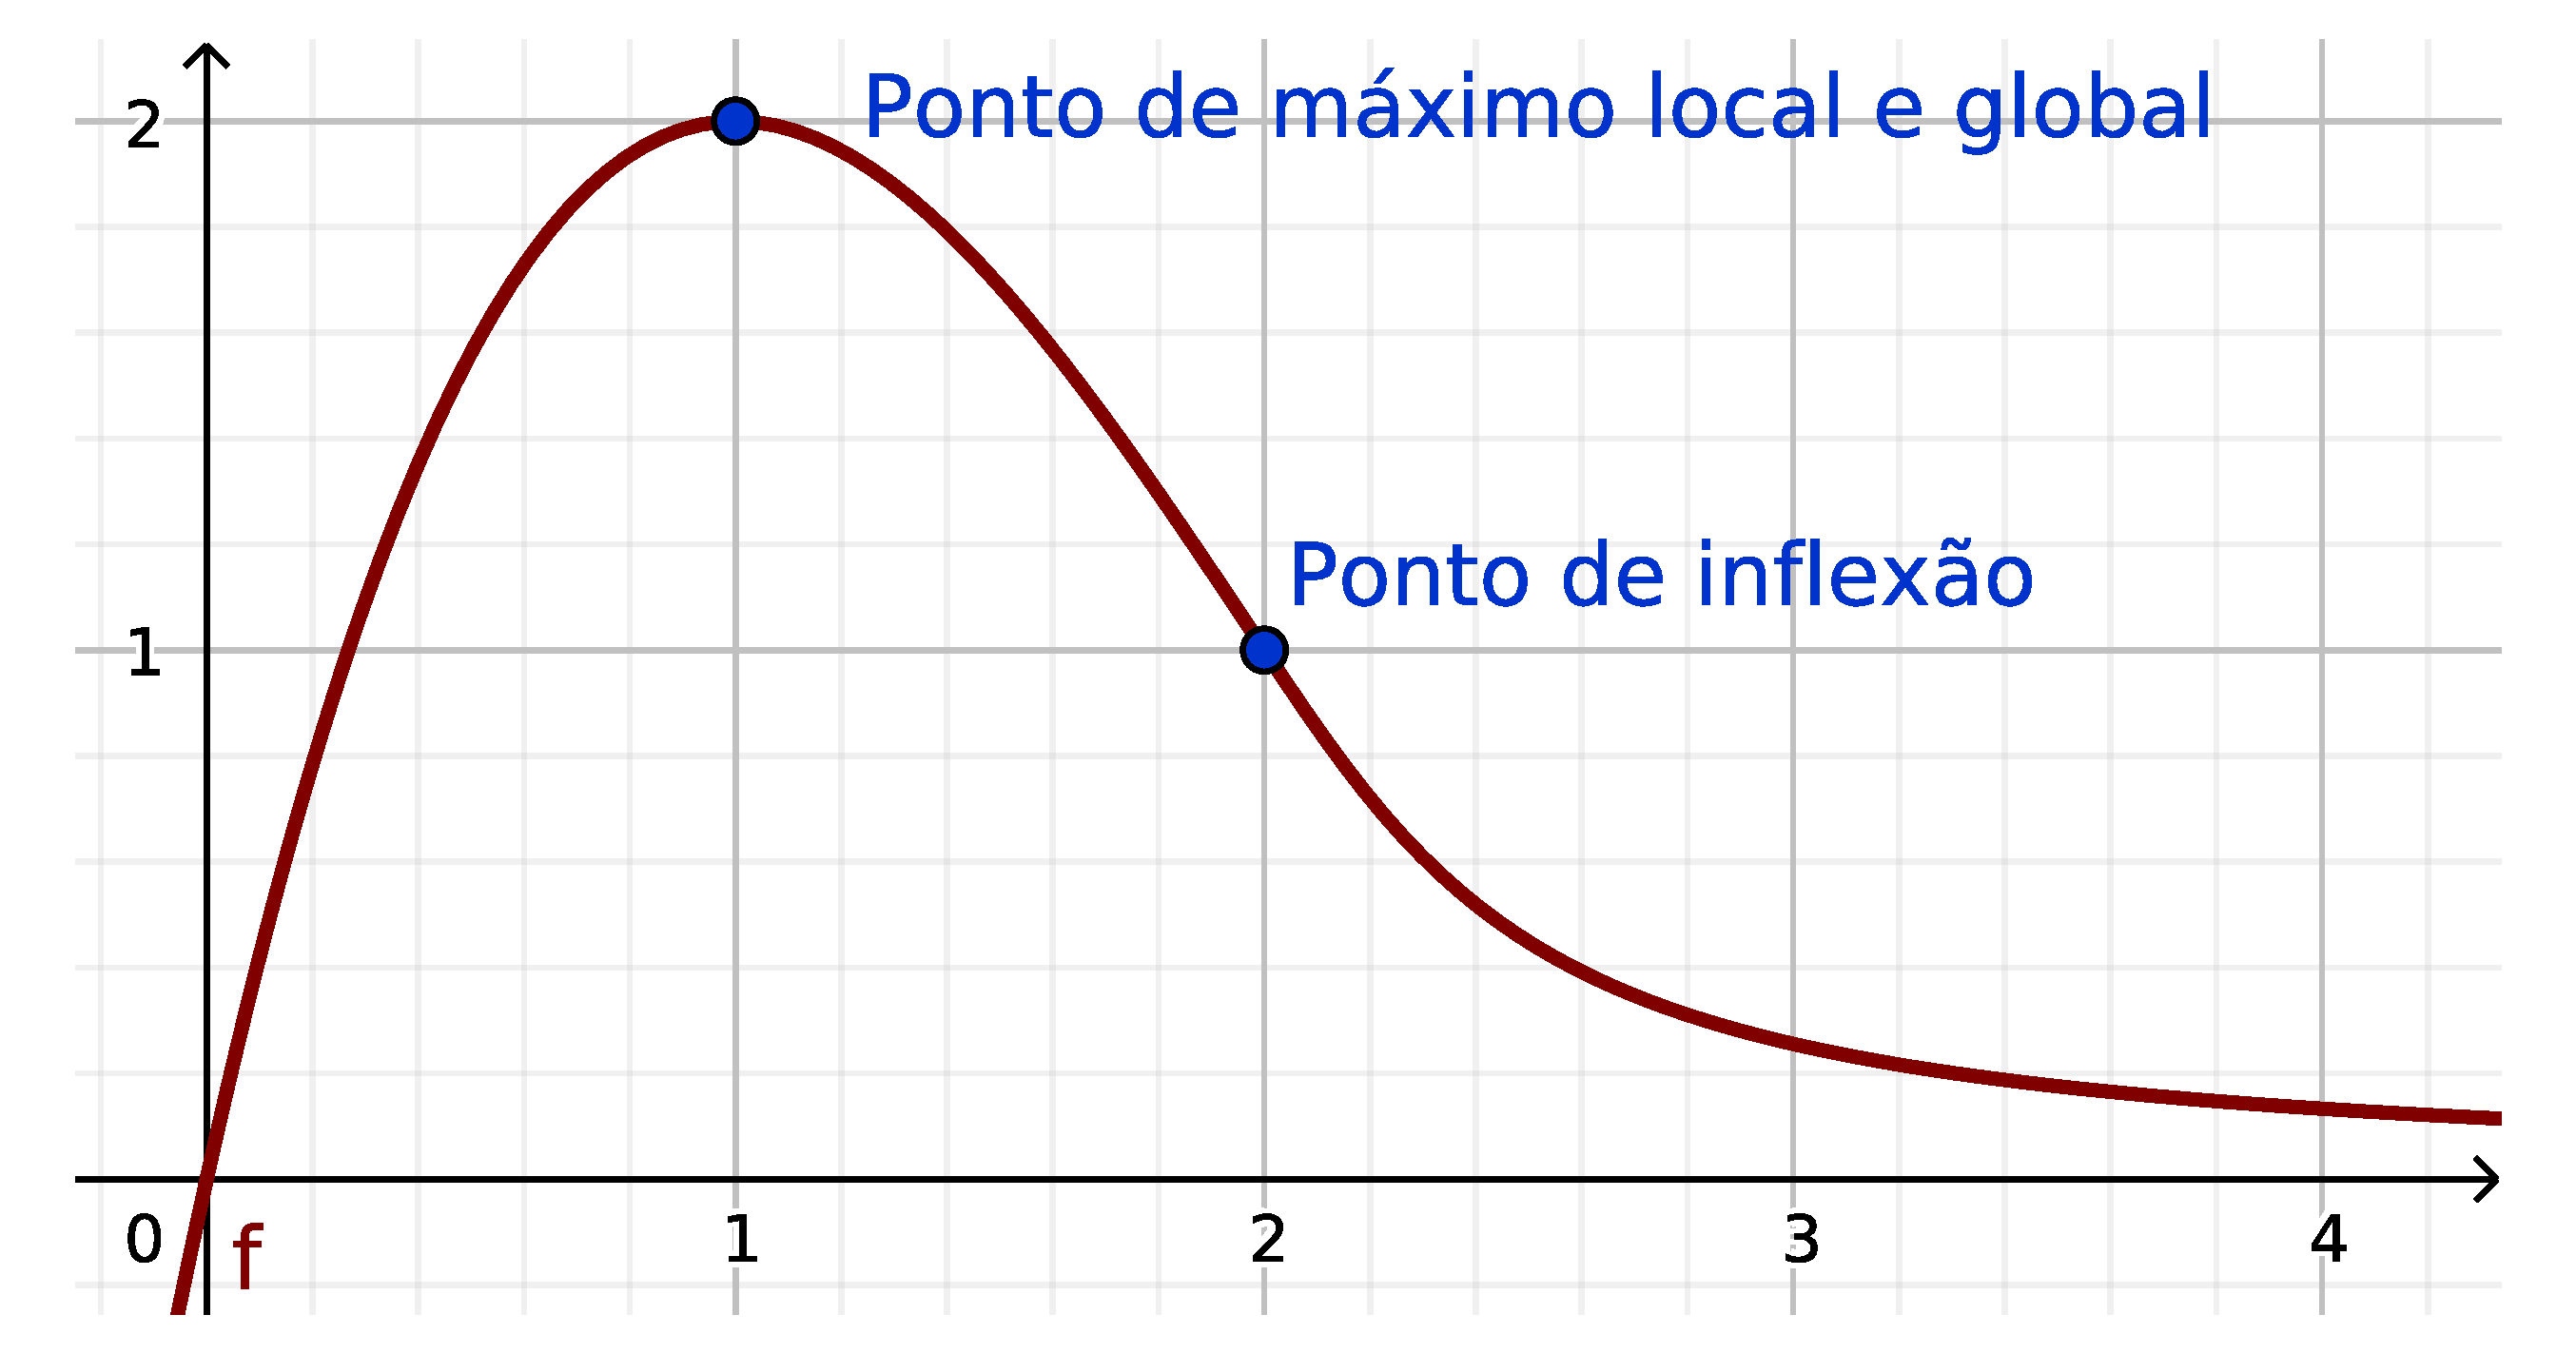
\includegraphics[width=0.5\textwidth]{img/prova-3-tads-graph}
\end{center}
\end{enumerate}


\Exercise[title={2,0}]
Obtenha todas as assíntotas oblíquas e verticais da função $g(x) = \dfrac{x^3 - 8x^2 + 21x - 18}{x^2 - 4}$.
\Answer Considerando que $x^2 - 4 = 0 \Leftrightarrow x = \pm 2$, é possível que $g$ tenha assíntotas verticais nessas abscissas. Para ter certeza, deve-se verificar se $g$ tende a $\pm \infty$ nestes pontos:
\[
  \lim_{x \to 2} \dfrac{\cancelto{0}{x^3 - 8x^2 + 21x - 18}}{\cancelto{0}{x^2 - 4}}
\stackrel{\text{L.H.}}{=}
  \lim_{x \to 2} \dfrac{3x^2 - 16x + 21}{2x}
= \dfrac{12 - 32 + 21}{4}
= \dfrac{1}{4}
\]
Logo, $x = 2$ \textbf{não é} uma assíntota vertical de $g$. Por outro lado,
\[
  \lim_{x \to -2} \dfrac{ \cancelto{-100}{x^3 - 8x^2 + 21x - 18} }{ \cancelto{0}{x^2 - 4}}
= \pm \infty
\]
Logo, $x=-2$ é uma assíntota vertical de $g$. Para as possíveis assíntotas oblíquas, observe que
\begin{align*}
  a = \lim_{x \to +\infty} \frac{g(x)}{x}
& = \lim_{x \to +\infty} \dfrac{ \cancelto{+\infty}{x^3 - 8x^2 + 21x - 18} }{ \cancelto{+\infty}{x^3 - 4x}}
\stackrel{\text{L.H.}}{=}
\lim_{x \to +\infty} \dfrac{ \cancelto{+\infty}{3x^2 - 16x + 21} }{ \cancelto{+\infty}{3x^2 - 4}} \\
& \stackrel{\text{L.H.}}{=}
\lim_{x \to +\infty} \dfrac{ \cancelto{+\infty}{6x - 16} }{ \cancelto{+\infty}{6x}}
\stackrel{\text{L.H.}}{=}
\lim_{x \to +\infty} \dfrac{ 6 }{ 6 }
= 1
\end{align*}
e que
\begin{align*}
b
& = \lim_{x \to +\infty} g(x) - a x
  = \lim_{x \to +\infty} \dfrac{ x^3 - 8x^2 + 21x - 18 }{ x^2 - 4 } - x \\
& = \lim_{x \to +\infty} \dfrac{ x^3 - 8x^2 + 21x - 18 - x^3 + 4x}{ x^2 - 4 }
  = \lim_{x \to +\infty} \dfrac{ -8x^2 + 25x - 18}{ x^2 - 4 } \\
& = \lim_{x \to +\infty} \dfrac{x^2 (-8 + 25/x - 18/x^2)}{ x^2(1 - 4/x^2) }
  = \frac{-8}{1} = -8
\end{align*}
Logo, $y = x-8$ é uma assíntota oblíqua de $g$ em $+\infty$. Um procedimento análogo mostra que esta reta também é uma assíntota em $-\infty$, mas isso também pode ser comprovado observando que
\begin{align*}
    \lim_{x \to -\infty} g(x) - (x - 8)
& = \lim_{x \to -\infty} \dfrac{ x^3 - 8x^2 + 21x - 18 }{ x^2 - 4 } - (x-8) \\
& = \lim_{x \to -\infty} \dfrac{ x^3 - 8x^2 + 21x - 18 - (x-8)(x^2 -4)}{ x^2 - 4 } \\
& = \lim_{x \to -\infty} \dfrac{ x^3 - 8x^2 + 21x - 18 - x^3+4x+8x^2-32}{ x^2 - 4 } \\
& = \lim_{x \to -\infty} \dfrac{ \cancelto{-\infty}{25x - 50} }{ \cancelto{+\infty}{x^2 - 4} }
 \stackrel{\text{L.H.}}{=}
 \lim_{x \to -\infty} \dfrac{ 25 }{ 2x } = 0,
\end{align*}
ou seja, a função $g(x)$ se aproxima da reta $y = x-8$ quando $x \to -\infty$.
\end{ExerciseList}

\begin{center}
BOA PROVA!
\end{center}

\newpage
\restoregeometry
\section*{Respostas}
\shipoutAnswer
\end{document}
